    %%%%%%%%%%%%%%%%%%%%%%%%%%%%%%%%%%%%%%%%%%%%%%%%%%%%%%%%%%%%%%%%%%%%%%
% How to use writeLaTeX: 
%
% You edit the source code here on the left, and the preview on the
% right shows you the result within a few seconds.
%
% Bookmark this page and share the URL with your co-authors. They can
% edit at the same time!
%
% You can upload figures, bibliographies, custom classes and
% styles using the files menu.
%
% If you're new to LaTeX, the wikibook is a great place to start:
% http://en.wikibooks.org/wiki/LaTeX
%
%%%%%%%%%%%%%%%%%%%%%%%%%%%%%%%%%%%%%%%%%%%%%%%%%%%%%https://v2.overleaf.com/project/5baac094de0904180e28e9b3%%%%%%%%%%%%%%%%%
\documentclass{tufte-handout}

%\geometry{showframe}% for debugging purposes -- displays the margins

\usepackage{amsmath}

% Set up the images/graphics package
\usepackage{graphicx}
\setkeys{Gin}{width=\linewidth,totalheight=\textheight,keepaspectratio}
\graphicspath{{graphics/}}

\title{How Factor Drive\texttrademark Works}
\author[Hugh Winkler]{Hugh Winkler}
\date{23 October 2018}  % if the \date{} command is left out, the current date will be used
% The following package makes prettier tables.  We're all about the bling!
\usepackage{booktabs}

% The units package provides nice, non-stacked fractions and better spacing
% for units.
\usepackage{units}

% The fancyvrb package lets us customize the formatting of verbatim
% environments.  We use a slightly smaller font.
\usepackage{fancyvrb}
\fvset{fontsize=\normalsize}

% Small sections of multiple columns
\usepackage{multicol}

% Provides paragraphs of dummy text
\usepackage{lipsum}

% These commands are used to pretty-print LaTeX commands
\newcommand{\doccmd}[1]{\texttt{\textbackslash#1}}% command name -- adds backslash automatically
\newcommand{\docopt}[1]{\ensuremath{\langle}\textrm{\textit{#1}}\ensuremath{\rangle}}% optional command argument
\newcommand{\docarg}[1]{\textrm{\textit{#1}}}% (required) command argument
\newenvironment{docspec}{\begin{quote}\noindent}{\end{quote}}% command specification environment
\newcommand{\docenv}[1]{\textsf{#1}}% environment name
\newcommand{\docpkg}[1]{\texttt{#1}}% package name
\newcommand{\doccls}[1]{\texttt{#1}}% document class name
\newcommand{\docclsopt}[1]{\texttt{#1}}% document class option name

\begin{document}

\maketitle% this prints the handout title, author, and date
% \textcopyright2018 Factor Technology LLC. All Rights Reserved.

\begin{abstract}
\noindent
Factor Drive\texttrademark solves the geosteering problem probabilistically.
It models everything in the system as random variables, and then  
calculates the probability of each possible configuration of those variables.
\end{abstract}

%\printclassoptions

In 2017 I published an article\cite{Winkler2017}  describing a way to
compute a geosteering interpretation. The core concept is that
you have to conceive of the geosteering problem as having probabilistic inputs and a probabilistic answer. 
That's the only way you can compute all the
possible geologic structures and wellbore trajectories that could explain the log
and survey measurements.
The article employs Bayesian networks to formulate and solve the probabilistic problem, but you
don't need to understand Bayesian networks to understand the probabilistic concepts and to get
a feeling for how Factor Drive works. 

The inputs to the geosteering problem are log and survey measurements that have uncertainty,
along with your uncertain geologic knowledge about the region you're drilling, and
an approximate engineering model for the shape of the wellbore.
We want to  discover the most probable geologic structure and 
the well position, while recognizing that other answers are possible. So there's 
uncertainty in the output as well.

For "uncertain" you can read "described by a probability distribution".
Think of a survey measurement of 89\textdegree $\pm$ 0.25\textdegree 
as a probability distribution with mean 89\textdegree and standard deviation 
0.25\textdegree. And think of the answers, estimates of the geologic structure and 
the well position, as probability distributions too. There's a most likely
configuration of these quantities, but there's a confidence measure around those answers too. 
This is what I mean by "conceive of the geosteering problem as having probabilistic 
inputs and a probabilistic answer".

\section{How It Doesn't Work}\label{sec:how-it-doesnt-work}
Factor Drive doesn't simulate the way people use a conventional geosteering program.
It doesn't try a lot of different geologic structures and wellbore trajectories, selecting
the configuration that gives the best correlation between the type log and the MWD gamma ray. The
interpretation that gives the best correlation may not be the most likely one.
Correlation is a good guide; under many common circumstances it does give you the best
interpretation, and it is a good QA tool. But the assumptions it requires are too limiting to use it to compute interpretations.
Correlation can fail if there are ambiguous, nearly identical features on the log; a fault can cause a misleading alignment. Mathematically, we'd say that the "best correlation" rule fails because the variables you're optimizing aren't normally distributed.

\begin{marginfigure}
  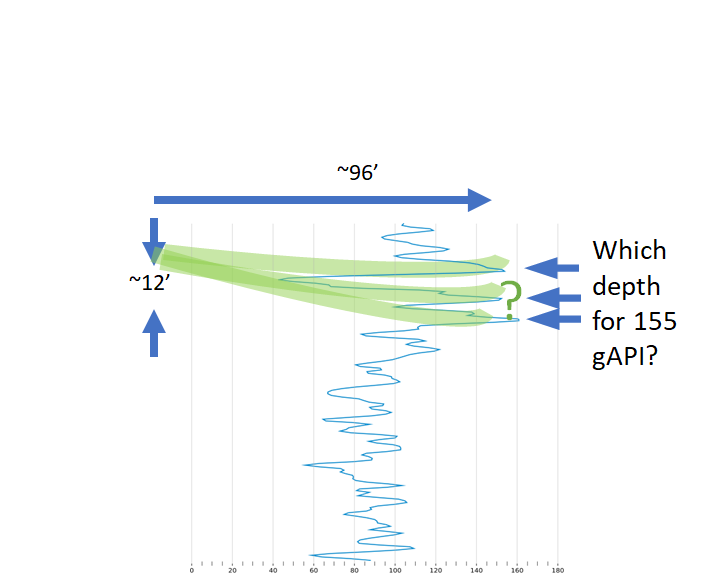
\includegraphics{which-depth-for-155-gapi.png}
  \caption{This gamma ray type log touches near 155 gAPI at three separate depths.}
  \label{fig:which-depth-for-155-gapi}
\end{marginfigure}

Geologists know how to work around these limitations. They use correlation as a guide, but overrule the numbers whenever geologic or engineering sense dictates. Factor Drive captures those heuristics as probability distributions.

\section{How It Works}\label{sec:how-it-doesnt-work}
\subsection{The Fundamental Problem of Geosteering}\label{sec:fundamental-problem}

Given a log value while drilling, what stratigraphic depth did it come from? That is the 
fundamental problem of geosteering. The answer to that question gives you the key piece of information you need
to estimate the true geologic structure depth and wellbore position.

\begin{marginfigure}
  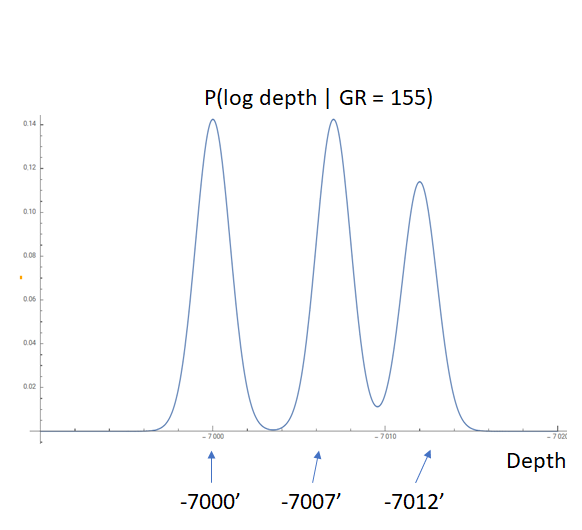
\includegraphics{probability-density-for-155-gapi.png}
  \caption{If we measure 155 gAPI, the log in figure \ref{fig:which-depth-for-155-gapi} implies
  a probability distribution. In this case there are three nearly equal candidates for the 
  stratigraphic depth.}
  \label{fig:probability-density-for-155-gapi}
\end{marginfigure}

If the only thing you know is that a GR reading of 155 gAPI came from somewhere in the depth range on figure
\ref{fig:which-depth-for-155-gapi}, the log tells you that the reading probably came from one of the three depths where the log reaches that value. By "probably", I mean we can represent that knowledge by a
probability distribution, as in figure \ref{fig:probability-density-for-155-gapi}. Factor Drive 
builds a probability distribution like this one for every MWD measurement.


\begin{figure*}
    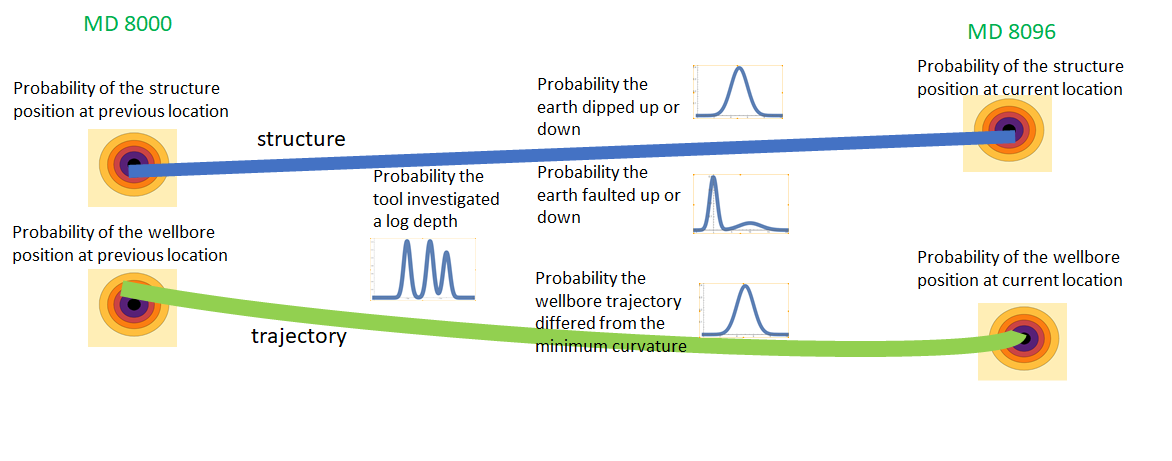
\includegraphics[width=\linewidth]{neighboring-stations.png}
    \caption{If we have estimates for the wellbore position and the structure depth at a previous
    position (8000 MD), then we combine the probabilities describing the dip, the faulting, and the
    change in wellbore position, with the probability for the stratigraphic depth from 
    \ref{fig:probability-density-for-155-gapi}, to estimate the wellbore position and
    structure depth at the current position (8096 MD).}
    \label{fig:neighboring-stations}
\end{figure*}

But we have more information (figure \ref{fig:neighboring-stations}). We have estimates for the wellbore depth and the structure depth 
at the previous survey position; we have surveys at the beginning and end of that segment; and we know
some constraints on the range of possible geologic dip and wellbore curvature in that interval. Before
running a computation, you tell Factor Drive a regional dip, or you give it a structure description;
along with that, you specify an uncertainty, in degrees of dip, that allows the algorithm some wiggle
room. You also specify, in degrees of inclination, the uncertainty in the directional surveys. The
minimum curvature rule gives a good first estimate of the change in well position between
the ends of the segment, but small survey errors can cause significant departures from that estimate.
In fact, the shape of the wellbore may not trace the minimum curvature arc of a circle: it 
may have a series of scalloped shapes as the driller slides and rotates to build curve. 

\begin{marginfigure}
  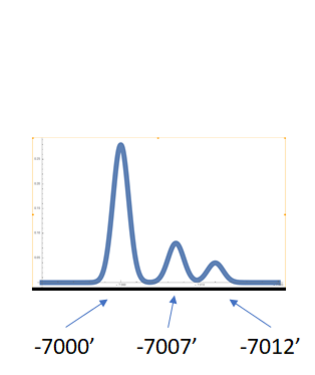
\includegraphics{so-you-adjust-your-probability.png}
   \caption{Our knowledge about the local dip and how much pipe can bend across a short interval 
  modifies the probability from figure \ref{fig:probability-density-for-155-gapi}}.
  \label{fig:so-you-adjust-your-probability}
\end{marginfigure}

All of that other information causes us to adjust our original probability for the 
depth. Factor Drive multiplies the probability functions together to modify the original
probability of figure \ref{fig:probability-density-for-155-gapi}. In figure \ref{fig:so-you-adjust-your-probability}, the additional information causes us to favor
the choice of 7000' as the most probable stratigraphic depth.

% \begin{figure}[h]
%     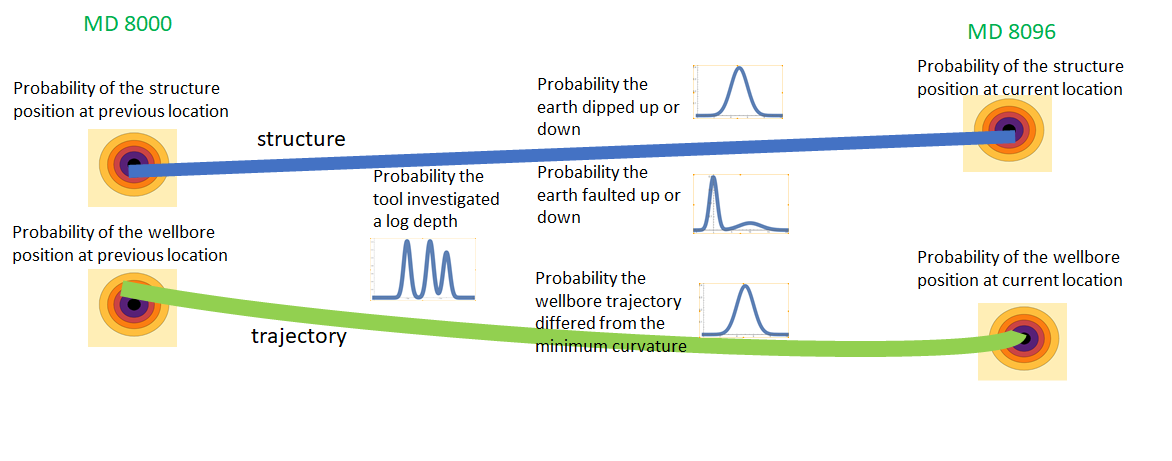
\includegraphics[width=\linewidth]{neighboring-stations.png}
%     \caption{If we have estimates for the wellbore position and the structure depth at a previous
%     position, then combining the probabilities describing the dip, the faulting, and the }.
%     \label{fig:neighboring-stations}
%     \setfloatalignment{b}
% \end{figure}

New log and survey measurements at the bit can can shed light on what's going on hundreds or thousands of feet back. We're looking for the overall most likely combination of structure and
well position, so we have to combine all the probabilities of all those variables (dip, fault,
inclination, and a few more we haven't mentioned), at all positions along the wellbore, to get
an updated overall picture of the joint probability (figure \ref{fig:the-answer}).
In practice, Factor Drive subdivides the trajectory into short segments,
much shorter than the usual 96-foot drill pipe stand length; it has a set of those
probabilities for each segment. For each new measurement at the bit, it has to multiply 
all of those thousands of probability functions together. It's an impossible computation, if
you approach it naively. It would require more bytes of computer memory than there are
atoms in the universe.

\begin{figure*}[h]
    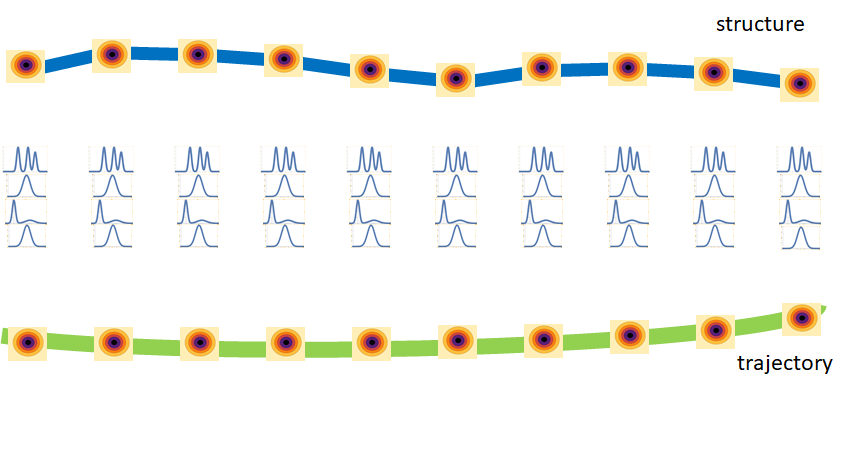
\includegraphics[width=\linewidth]{the-answer.png}
    \caption{
    The final geosteering answer must account for all the probabilities and constraints
    along the whole wellbore, simultaneously, to calculate the most likely structure and
    wellbore trajectory.
    }.
    \label{fig:the-answer}
\end{figure*}

The Bayesian network is simply a way to reduce the size of that computation. 
Bayesian networks arrange those probability functions into a graph that recognizes
the dependencies among them. By using the network to guide the order in which you multiply
and sum the probabilities, you never have to hold more than a handful of probability 
functions in computer memory at any one time. Factor Drive's innovation is that we designed
a network specifically for the geosteering problem that enables the computation to run
on the kinds of computers available today, quickly enough to give you answers in the
time it takes to drill a stand of pipe.

\bibliography{sample-handout}
\bibliographystyle{plainnat}


\end{document}